\section{Results}
\label{sec:results}

In this section we show the estimated number of events and uncertainty from each background. The \pt spectrum and particle flow \met of our selected candidate events in various cut regions and estimated backgrounds can be seen in the following subsections.

%Since data are compatible with the standard model expectation, upper limits on new physics processes cross sections are set.

We adopt the official CMS statistical higgs combination tool\cite{higgstool}, used for upper crossection limits. The method adopted is asymptotic $CL_S$ \cite{CLs} and systematic uncertainties are introduced as nuisance parameters following log-normal distributions. Nuisances arising from jet/met energy scale, xsec normalizations and pileup are considered. The photon energy scale uncertainty is also introduced as nuisance parameters following log-normal distributions. 


\subsection{Model Independent Limits} \label{sec:shared}
Due to the multitude of signals one can apply to this region, we show the results for general cuts that are shared between all $\gamma + \met$ final signals. In addition to the kinematic requirements and photon ID requirements, we apply spike cleaning cuts and lepton vetos. Due to advanced fake \met rejection cuts having non trivial efficiencies, we have decided to apply easier angle based cuts to reject fake \met events. These cuts will be easier for a theories to implement and still provides rejection to events with non intrinsic \met. Explicitly we reject the events with more than 1 non pile up jet with $\PT>30 GeV$, and events with jets back to back with a photon, $\Delta\Phi$(Jet,$\gamma$) $> 2.5$. The yields and the distriubtions are shown in Table \ref{tab:model} and Fig. \ref{fig:model}.



\begin{table}[!hp]                                                                  
\center    
{          
\begin{tabular}{|c|c|}                                                             
\hline     
Process & \# of Events \\                                                              
\hline     
$\gamma +$ jets                          & $(313 \pm 50 ) x 10^3$ \\
${\rm jet}\rightarrow \gamma$        & $(906 \pm 317 ) x 10^2$ \\
${\rm e} \rightarrow \gamma$         & $(1035 \pm 62 ) x 10^1$ \\
$W(\to \ell\nu)+\gamma $                 &  $2239 \pm 111$ \\
$Z( \to \nu \bar{\nu} )+\gamma    $      & $ 2050 \pm 102$ \\
Other                                    &  $1809 \pm 91$ \\
\hline
Total background                       &   $(420 \pm 82 ) x 10^3$ \\
\hline
Data                                   &  $442 x 10^3$   \\
\hline     
\end{tabular}  
\caption{Comparison of event yields for background, derived from MC simulation and data-driven methods, after model independent selection compared to the data yieldsx.}
\label{table:model}                                                                
}          
\end{table}

\begin{figure}[!hp]
\centering
{\includegraphics[scale=0.4]{Unblinding/ModelIndep/StackedHisto_Pho_Pt.pdf}}
{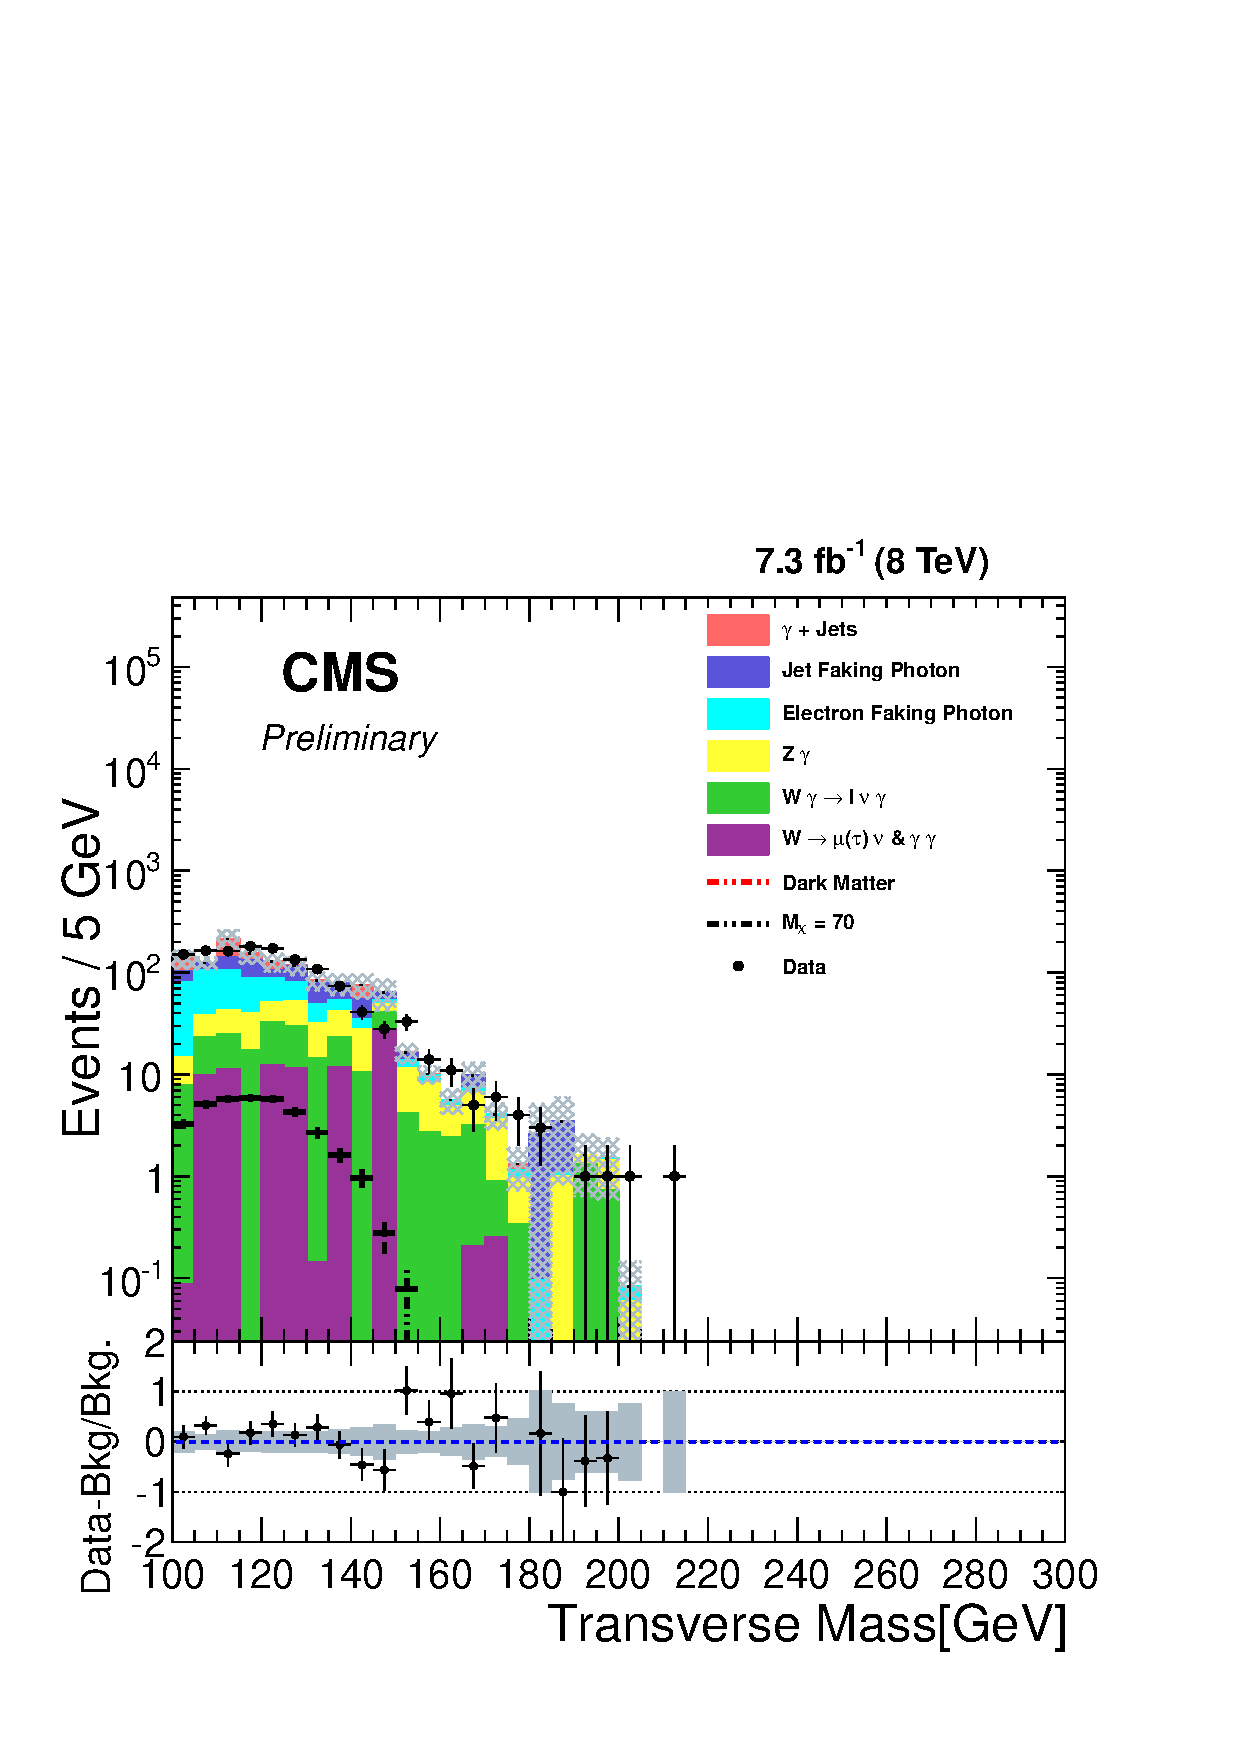
\includegraphics[scale=0.4]{StackedHisto_MT.pdf}}\\
{\includegraphics[scale=0.4]{StackedHisto_MET.pdf}}
\caption{The $\gamma$ $\PT$ ,$\met$ and MT distributions for model independent limit setting selection.}
\label{fig:model}
\end{figure}

The provided limits are only valid for the selection we have used, therefore, we extracted the efficiencies of our cuts. Theorist, should ideally also smear their generator level \met to mimic the reconstructed level \met distributions. this could be done using the resolution parameterization shown earlier in the note. The underlying assumption when extracting the efficiencies is that, efficiency for a particular selection does not depend on the kinematics of a specific model. We have therefore used cuts that do not depend on the kinematics of a specific model ($\Delta\Phi$ cut instead of mht minimization). The overall efficiency for photon identification is provided in the latest EG Report. We have already discussed in detail the trigger turn on efficeincies. And these are all the efficiencies need to interpret any signal model usign these limits. The expected limits as a function of \met and transverse mass can be seen in Fig. \ref{fig:model_lim} for various \met and transverse mass cuts.

\begin{figure}[!hp]        
\centering                
{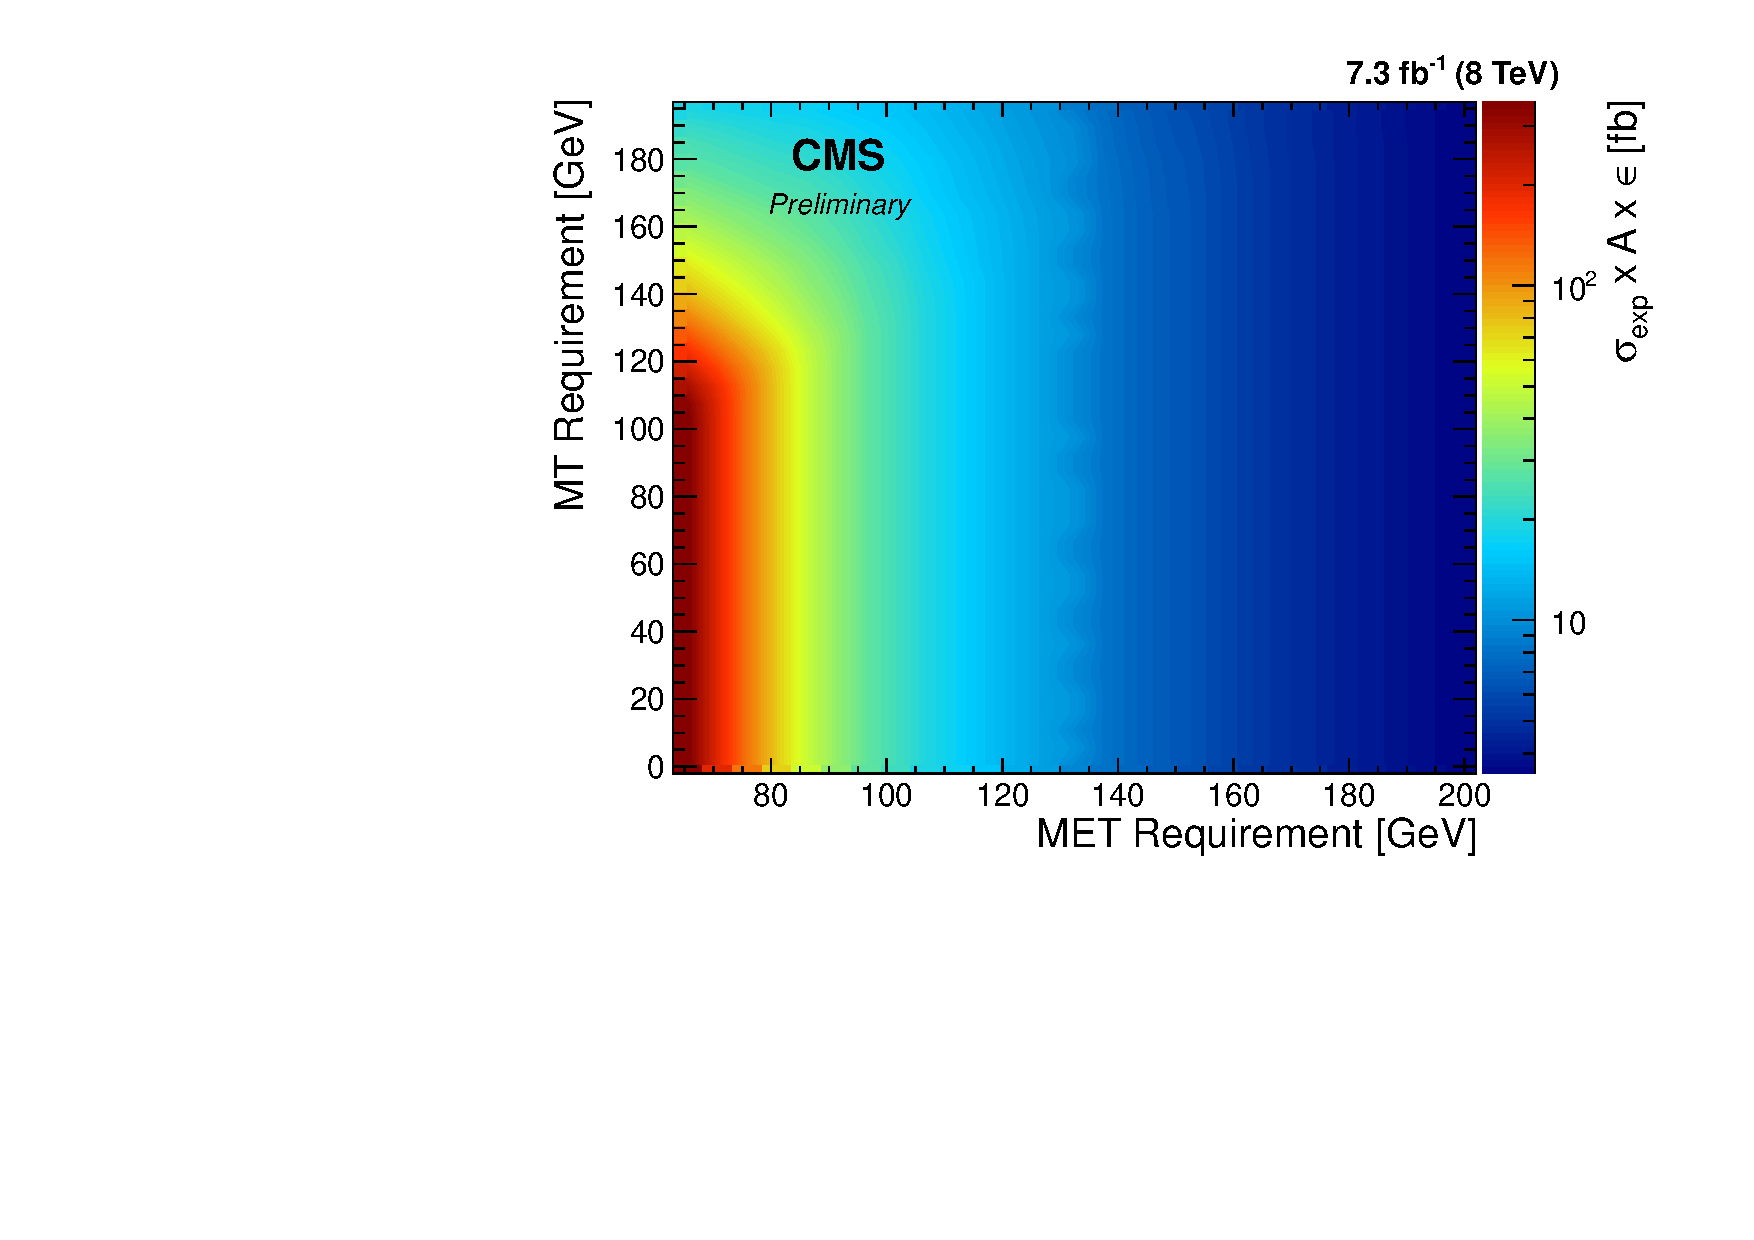
\includegraphics[scale=0.4]{2d_final_expected.pdf}}
{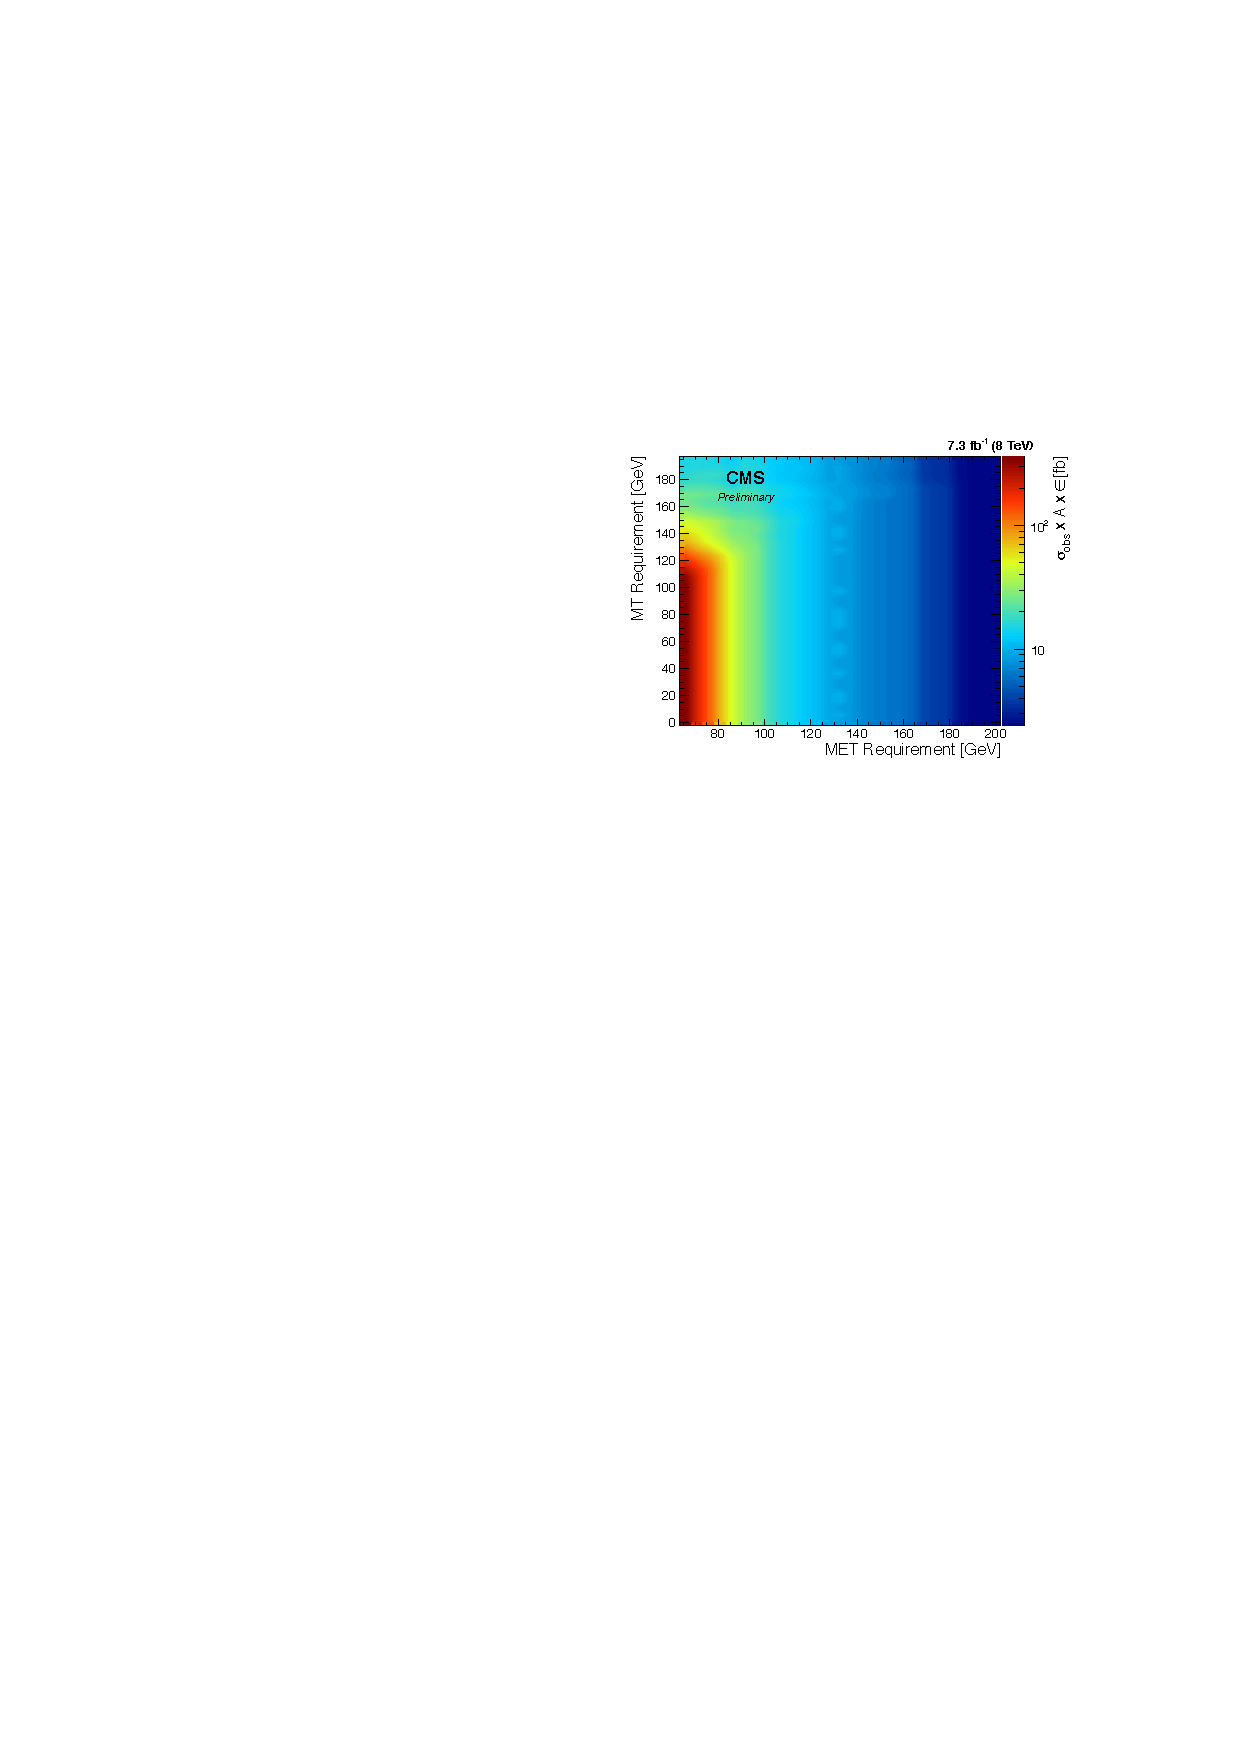
\includegraphics[scale=0.4]{2d_final_observed.pdf}} \\
{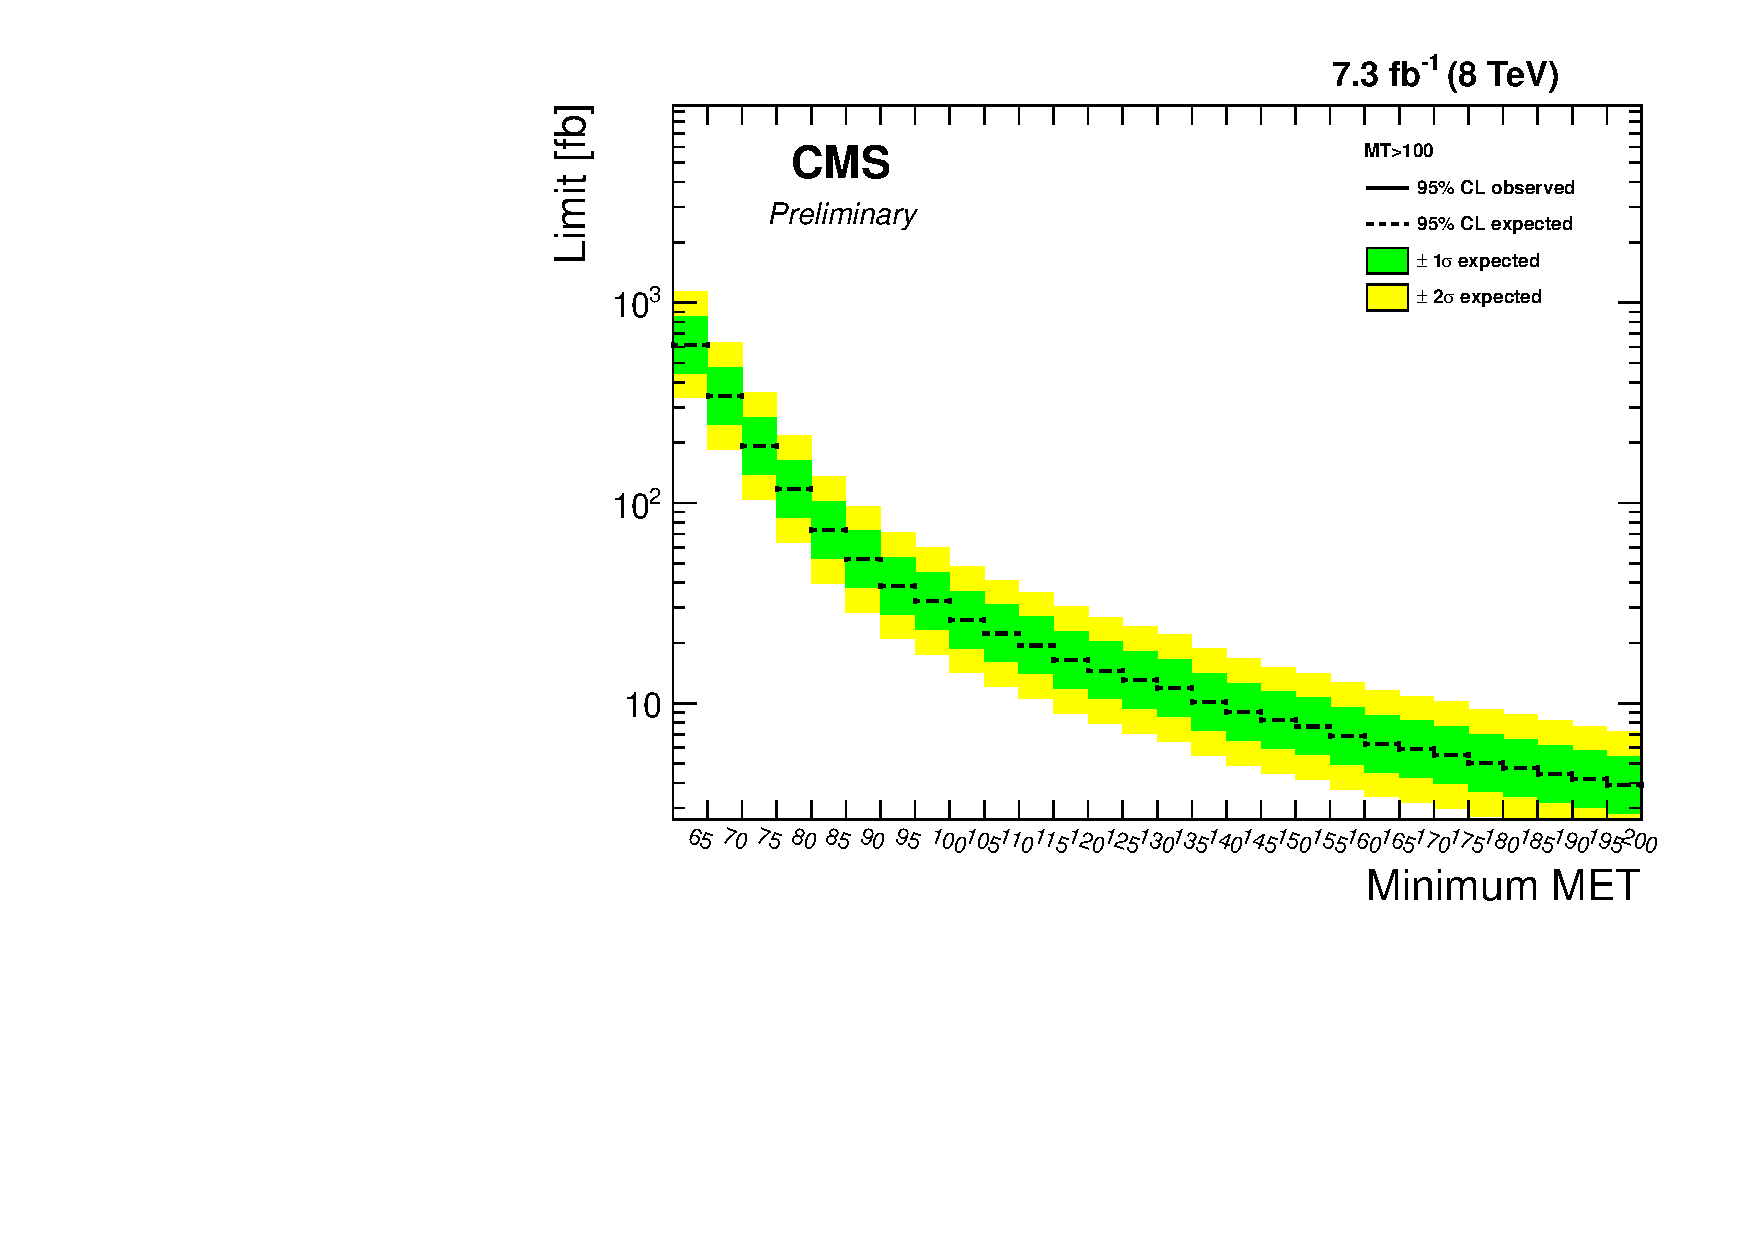
\includegraphics[scale=0.4]{LimitPlotVsMET_MT100.pdf}}
\caption{ The 95$\%$ CL upper limit on $\sigma \times BR\times A\times\epsilon$ for (a) different $M_{T}$ and low \met thresholds, (b) high \met thresholds,  and (c) for $M_{T}> 100$ GeV as function of \met.}
\label{fig:model_lim}
\end{figure}

\subsection{SUSY Higgs Limits}

The SUSY Higgs analysis phase space requires additional signal specific cuts on the photon \pt. The lower and upper bounds of the photon \pt are motivated by the theory to eliminate other background processes that would arise from supersymmetric models. Contaminations coming from these backgrounds (although BSM), will have to be removed as they are not simulated as a part of the standard model backgrounds. The lower bound of the photon \pt cut of 45 \GeV is motivated to eliminate the  process involving an on-shell $Z$ boson which is relevant only for $m_{\chi} <  m_Z$. The diagram for this process is shown in Fig.~\ref{fig:lowerbound} where the $Z$ boson gives rise to photons with lower \pt ($p_{T,\gamma} <  m_Z/2$) than the one involving the Higgs boson, for which $p_{T,\gamma} <  m_h/2$. On the other hand, one process which does not arise from the simplified model but which in general contributes to this final state in low scale SUSY breaking models is the non-resonant process involving a squark $t$-channel exchange, shown in Fig. \ref{fig:upperbound}. This process is dominant with respect to the resonant processes in the region where $p_{T,\gamma} >  m_h/2$.	Therefore we  will only consider the region $p_{T,\gamma} <  m_h/2$.

\begin{figure}[!hp]
\centering
{\label{fig:lowerbound}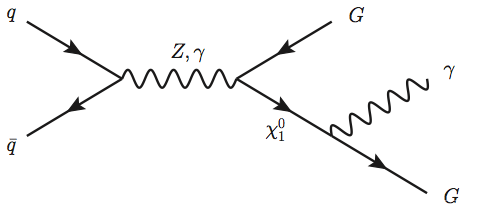
\includegraphics[scale=0.35]{analysis_figs/lower.png}}
{\label{fig:upperbound}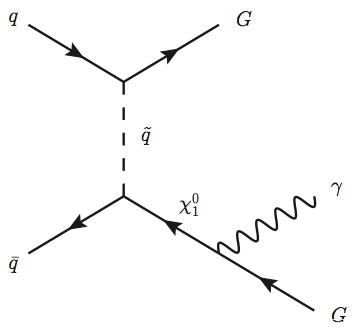
\includegraphics[scale=0.3]{analysis_figs/upper.png}}
\caption{Feynman diagrams corresponding to the resonant contributions to the final state with a photon + \met in the simplified model [a] and $t$-channel squark exchange contribution to the final state with a photon + \met [b]}
\end{figure}

We also required Minimized \met $> 45 $\GeV and Met Significance $> 20$. The transverse mass of the $\gamma + \met$ system is required to be greater than 100 \GeV. The event yields corresponding to this selection is shown in Table\ref{tab:exoh}. Where Fig. ~\ref{fig:exoh} shows the distributions for $\gamma$ \pt and \met after all the model specific cuts.

\begin{table}[!hp]
\center
{
\begin{tabular}{|c|c|}
\hline
Process & Estimate \\
\hline
$\gamma +$ jets                          & 179 $\pm$ 28 \\
${\rm jet}\rightarrow \gamma$        & 269 $\pm$ 94 \\
${\rm e} \rightarrow \gamma$         & 355 $\pm$ 28 \\
$W(\to \ell\nu)+\gamma $                 &  154 $\pm$ 15 \\
$Z( \to \nu \bar{\nu} )+\gamma    $      &  182 $\pm$ 13 \\
Other                                    &  91 $\pm$  10 \\
\hline
Total background                       &   1232 $\pm$ 188 \\
\hline
Data                                   &  1296  \\
\hline
\end{tabular}
\caption{Expected yields after the susy higgs selection cuts.}
\label{tab:exoh}
}
\end{table}

\begin{figure}[!hp]
\centering
{\label{fig:QCDPt}\includegraphics[scale=0.4]{Unblinding/Susy/StackedHisto_Pho_Pt.pdf}}
{\label{fig:QCDMET}\includegraphics[scale=0.4]{Unblinding/Susy/StackedHisto_MET.pdf}}
\caption{The $\gamma$ $\PT$ and $\met$ distributions for the susy higgs selection. }
\label{fig:exoh}
\end{figure}

%The acceptance and the efficiency for the signal samples we have considered are shown in Table~\ref{tab:acc}. 
It must be noted that part of the signal is rejected due to the fake \met rejection, especially the \met significance cut, has a big effect on signal acceptance. However, due to its power to reject a large amount of background, the analysis becomes more sensistive to the signal with the presence of this cut. We produce the first  upper limits on $\sigma x BR$ and the ratio of this product over the SM Higgs production cross section as a function of different $M_{\PSGczDo}$ values.

\begin{figure}[!hp]
\centering
{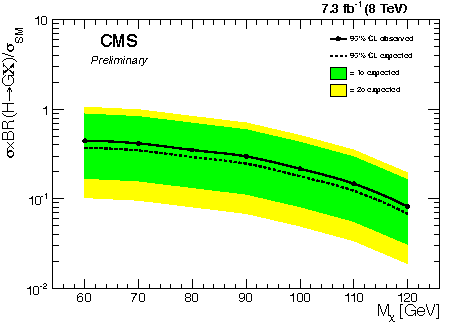
\includegraphics[width=0.45\textwidth]{ratio_log.pdf}}
{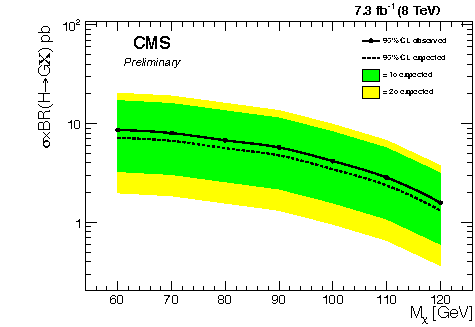
\includegraphics[width=0.45\textwidth]{xsec_log.pdf}}
\caption{ Expected 95\% CL upper limits on $\sigma x BR$ and the ratio of this product over the SM Higgs production cross section as a function of different $M_{\PSGczDo}$ values. The uncertainty on the expected limit at 1$\sigma$ and 2$\sigma$ levels are shown as yellow and green bands, respectively. }
\label{fig:limit_higgs}    
\end{figure}


%\subsection{Dark Matter Limits}
%Work ongoing.. Stayed tuned..
%\subsection{Dark Photon Limits}
%Work ongoing.. Stayed tuned..
